	\subsection{Python, Primary Programming Language}
	\par Python is an interpreted, interactive, object-oriented programming language. It incorporates modules, exceptions, dynamic typing, very high-level dynamic data types, and classes. Python combines remarkable power with very clear syntax. It has interfaces to many system calls and libraries, as well as to various window systems, and is extensible in C or C++. It is also usable as an extension language for applications that need a programmable interface. Finally, Python is portable: it runs on many Unix variants, on the Mac, and on Windows 2000 and later.
	\par We will use Python to control each module via the coordinator XBee module that will be attached to a PC. Its versatility provides the ability to interface lower level controls on the XBee with a high level graphical interface all in one language. 
	\par A readily available python package allows for easy interfacing with the camera unit. This package provides a pure Python interface to the Raspberry Pi camera module for Python 2.7 (or above) or Python 3.2 (or above). It can configure resolution and give different dimensions to the video or picture files. It can also take photos under varying conditions if given the right parameters for a camera to take a good picture in a variety of different conditions including poor lighting. 
	The code for the camera is as follows:
	\begin{lstlisting}
	# A test of the cameras functions
	from time import sleep
	from picamera import PiCamera
	
	camera = PiCamera()
	camera.capture('/home/pi/Desktop/test.jpg')  #saves camera picture to file location specified
	
	
	# Camera trigger implementations
	import RPi.GPIO as GPIO
	from picamera import PiCamera
	from time import sleep
	GPIO.setmode(GPIO.BOARD)
	GPIO.setup(16, GPIO.IN, pull_up_down=GPIO.PUD_DOWN) #Pull down to make pin read active high
	GPIO.input(16) #pin 16 being read
	if GPIO.input(16):
	camera = PiCamera()
	camera.capture('/home/pi/Desktop/test.jpg')
	print('input high/camera on')
	else:
	camera = PiCamera()
	camera.capture('/home/pi/Desktop/testfail.jpg')
	print('input low/camera off')
	GPIO.cleanup()
	\end{lstlisting}
	\subsection{Creating the Wireless Network between the Coordinator and Router modules}
	\par We wanted to create a wireless network between the coordinator and router modules this time. Firstly, we started off with soldering our XBee Explorer to connect our router modules on top of them. The reason we chose Xbee Explorer was because it will allow us to solder the input power voltage and the output pins that will be connected to the sensors. We used the application XCTU to help us set up each Xbee as a coordinator or router modules. We first set our coordinator in API mode that will allow us to communicate directly with the sensors via router modules. At the same time, we set the other three router modules to be in a AT or Transparent mode. This will allow sensors to send data directly to the coordinator. We also made sure all the XBee modules used the same Channel and Personal area network (PAN) ID. 
	\begin{figure}[h]
		\centering
		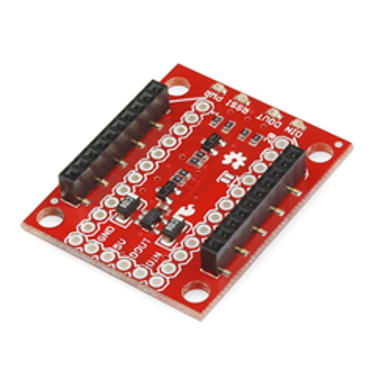
\includegraphics[width = 0.3\textwidth]{xbeeMiniExplorer.png}
		\caption{Small XBee interface to be used in each module}
	\end{figure}
	\subsection{Controlling the Router XBee with XCTU Remote AT Command}
	\par We decided to test our router XBee remotely by sending some AT Commands. We used the XCTU application to first create the Remote AT Command to turn on and off pin 18 of the router XBee. To see if we receive any output, we put an LED to see if the pin was turned on or not. In the figure below you can see the LED turning on and off via Pin 18 of the XBee device. The pictures help visualize what the pin is doing corresponding to the LED.
	\begin{figure}[h!]
		\centering
		\begin{subfigure}[t]{0.22\textwidth}
			\centering
			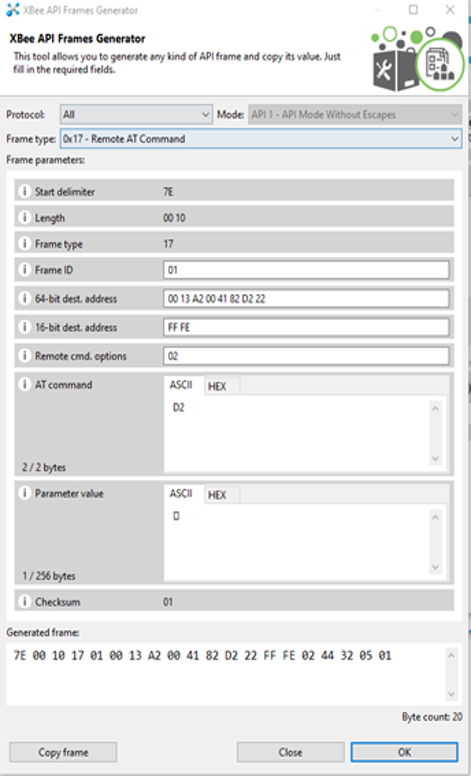
\includegraphics[width=\textwidth]{xbeeXctu1.png}
			\caption{Turn On Pin 18}
		\end{subfigure}
		\begin{subfigure}[t]{0.22\textwidth}
			\centering
			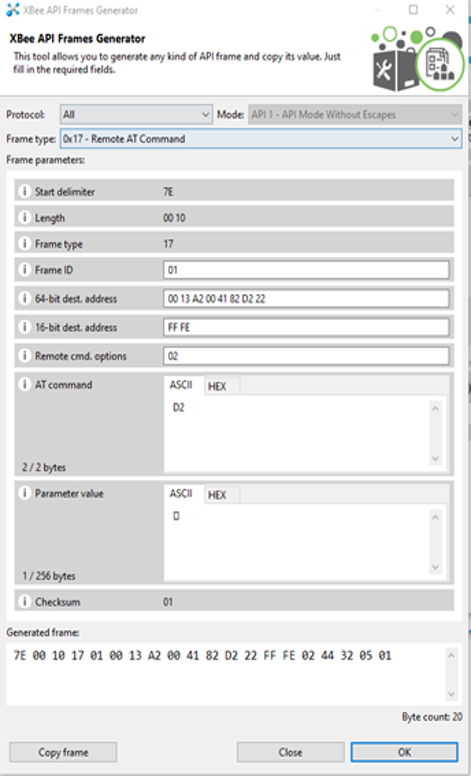
\includegraphics[width=\textwidth]{xbeeXctu1.png}
			\caption{Turn Off Pin 18}
		\end{subfigure}
		\caption{Simple LED activation over 802.15.4}
	\end{figure}
	\begin{figure}[h!]
		\centering
		\begin{subfigure}[t]{0.45\textwidth}
			\centering
			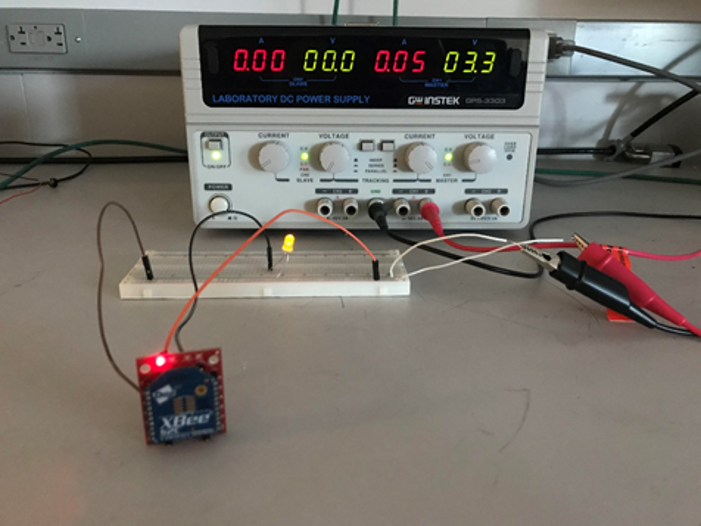
\includegraphics[height=1.5in]{ledRemoteTest.png}
			\caption{LED on via pin 18}
		\end{subfigure}
		\begin{subfigure}[t]{0.45\textwidth}
			\centering
			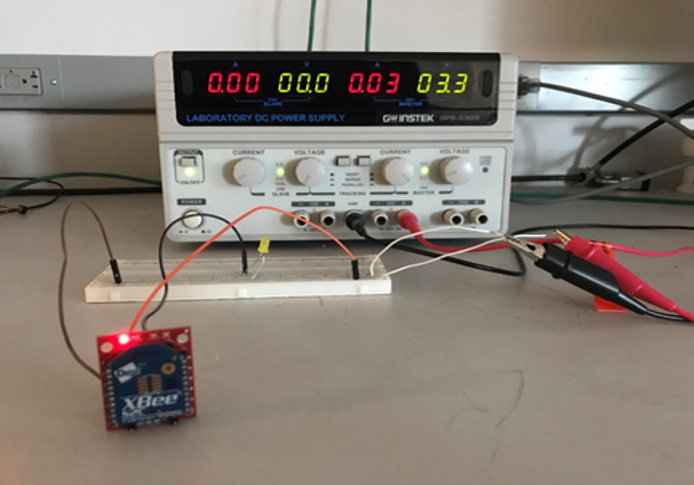
\includegraphics[height=1.5in]{ledRemoteTestOFF.png}
			\caption{LED off via pin 18}
		\end{subfigure}
		\caption{Simple LED activation over 802.15.4 (2)}
	\end{figure}
	\subsection{XBee Digital In/Out setup \textit{(DIO)}}
	\par The XBee devices have the capability to detect a change in a digital input signal. This edge detection allows the remote motion sensing module to transmit its data only if the signal changes. The coordinator will receive two packets, the first being a reading of logic high, the second being a reading of logic low once the sensor has stopped detecting any movement. In this way the unit does not need to send samples at a continuous rate, which saves power.
	\par To enable the change detection feature on DIO3, we need to set the hexadecimal value in the setting DIO change detect to 0x4. As seen on the right side of Figure \ref{fig:changeDet} this will enable the change detection on bit 2 only, which corresponds to DIO3. 
	\begin{figure}[h]
		\centering
		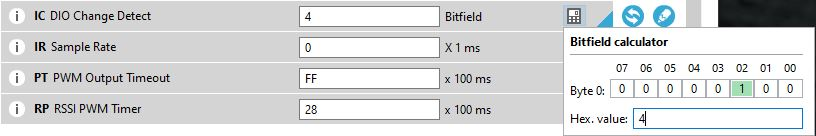
\includegraphics[width=\linewidth]{changeDetect.JPG}
		\caption{Change detection parameters in XCTU}
		\label{fig:changeDet}
	\end{figure}
	\par When initially attempting to read data from the XBee's DIO pin, the value read would always read high. This reading was verified with a multimeter as well as on the scope. After some trouble shooting it was discovered that the issue lie in the I/O settings of the XBee, which has the ability to pull its digital inputs or outputs high or low based on a bit mask. 
	\begin{figure}[h]
		\centering
		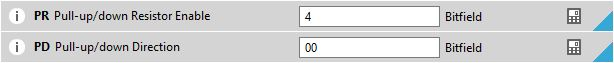
\includegraphics[width=\linewidth]{bitMask.JPG}
		\caption{Bit masking settings for pull-up/pull-down resistors.}
		\label{fig:bitMask}
	\end{figure}
	\par In XCTU the mask had been set to pull all DIO pins high, which was not allowing a low input to be seen. Once re-masked, pulling the DIO pin used for the sensor reading down by default, the values were read correctly.
	
	\subsection{Digital I/O Interfacing with Python}
	The next step was to interact with the system through via python. After some initial testing of functions and learning the syntax a small GUI (Figure \ref{fig:motGui}) was created to display red when tripped and green when no movement was present. 
	\begin{figure}[h]
		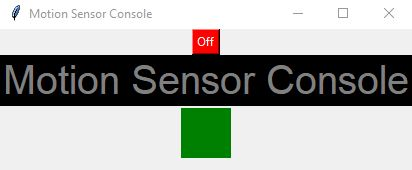
\includegraphics[width=\linewidth]{motionGui.jpg}
		\caption{Motion Sensor Interface}
		\label{fig:motGui}
	\end{figure}
\newpage
	\begin{lstlisting}
		# setup gui elements ---------
		
		window = tk.Tk(screenName="Test Name", baseName=None, className='Tk', useTk=1)
		window.title("Motion Sensor Console")
		motion_canvas = tk.Canvas(window, bg="green", width=50, height=50)
		btn_ON_OFF = tk.Button(window,
							   activebackground="grey",
							   text="Off",
							   fg='white',
							   bg='red'
							  )
		# window title banner
		window_banner = tk.Label(window,
								 text="Motion Sensor Console",
								 fg='grey',
								 bg='black',
								 relief="solid",
								 font=("Arial", 30, "normal")
								)
	\end{lstlisting}
		Then, by establishing a serial connection with the coordinator, the whole network can be controlled and modified from a python program. Reading the digital input from the remote sensor, its is converted into a usable format, and if a rising edge was detected the program enter the triggered state and display a a red block. When a falling edge is received, the program will reset to a normal state. 
		\begin{lstlisting}
			def get_motion_status(red_time):
				data_raw = ''
				initial_red_time = 0
				ser1 = serial.Serial('COM3', 9600, timeout=1.75)
				data_raw = ser1.read(14)
		\end{lstlisting}
		\par When using a GUI in python the window runs in an infinite loop, constantly updating. This prevents the program from executing anything while the \textit{"mainloop()"} is running. To avoid this issue. The gui will setup the window environment and then enter a recursive function that reads and interpenetrates the digital data being received and updates the window elements accordingly. 
		\begin{lstlisting}
			window_banner.pack()
			motion_canvas.pack()
			print("re-paint")
			window.update()
			print("set window interrupt")
			window.after(0, get_motion_status()) # recursive function
		\end{lstlisting}
		\par If the remote module was sending samples at a constant rate this is much simpler, missed packets are less of a concern. The change detect digital IO configuration will only send a data packet when an event occurs. This means that the python program must spend most of its time waiting for data to arrive from the serial port. By setting a timeout in the serial setup, the program will wait for data for a set time before executing the rest of the loop. If the timeout was indefinite the window would not update properly. If the timeout is too short, the program will miss packets that arrive while the rest of the function is executing. With a timeout slightly less that the 2 second high-time of the sensor itself, the program spend the majority of its time listening for data and will miss very few data transmissions, while still updating the window elements at a reasonable rate.
		\begin{lstlisting}
			if data_raw == '':
				ser1.close()
				window.after(0, get_motion_status())
				window.update()
			else:
				try:
					data_hex = binascii.hexlify(data_raw).decode('utf-8')
					D2 = data_hex[22:26]  # extract desired bits
					base_ten_val =int(D2, 16)
					# print("this sample:")
					print(base_ten_val)  # view data
				
				except ValueError:
					# print("caught valueError")
					ser1.close()
					# print("re-paint")
					window.update()
				
				else:
					print("Data received")
					if base_ten_val == 4:
					print("set indicator: red")
					motion_canvas.config(bg="red")
					print("re-paint")
					initial_red_time = time.now()
					window.update()
					elif base_ten_val == 0 or '':
					print("set indicator: green")
					motion_canvas.config(bg="green")
					print("re-paint")
					initial_red_time = 0
					window.update()
				finally:
					ser1.close()
					# print("re-paint")
					window.update()
					# print("set window interrupt")
					window.after(0, get_motion_status())
		\end{lstlisting}
		\begin{figure}[h]
			\centering
			\begin{subfigure}{0.4\textwidth}
				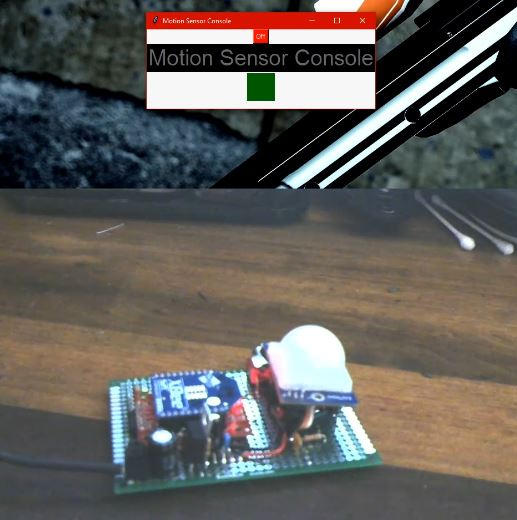
\includegraphics[width=\textwidth]{motionOff.JPG}
				\caption{Safe}
			\end{subfigure}
			\begin{subfigure}{0.4\textwidth}
				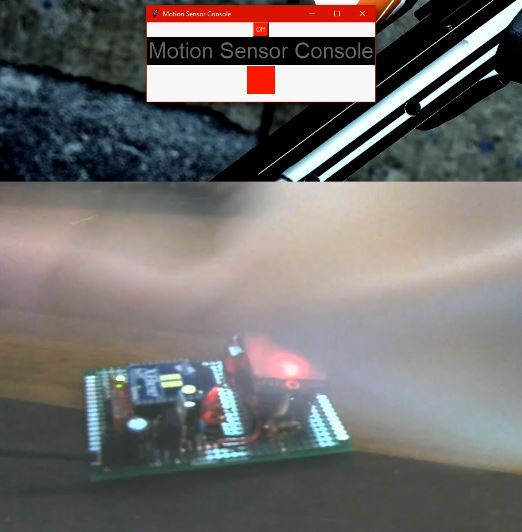
\includegraphics[width=\textwidth]{motionOn.JPG}
				\caption{Triggered}
			\end{subfigure}
		\caption{Motion Sensor GUI functionality}
		\label{fig:motionFunc}
		\end{figure}
		\par to account for any data that is missed a contingency was added to the program such that if the program is in the "tripped" state for too long it will automatically reset to "safe." If the sensor is being tripped it will be set to the "tripped" state again almost immediately. Remaining tripped for too long indicate that a rising edge was received but a falling edge was not. If no movement occurs after a missed falling edge the program would remain in the tripped state indefinitely.
		\begin{lstlisting}
			delta_t = time.now() - initial_red_time
			threshold_time = time.time(0, 0, 10)    # threshold for missed low == 10 sec
			
			if delta_t - threshold_time < 0:
				"""IF time after a high signal received exceeds 10 seconds, reset. If a falling edge missed program will remain high until the falling edge of subsequent trigger. If tripped value will return to tripped state on the next loop until 10 seconds have passed again. """
			
				print("set indicator: green")
				motion_canvas.config(bg="green")
				print("re-paint")
				initial_red_time = 0
				window.update()
		\end{lstlisting}
		
	
	\subsection{Controlling XBee module using Python}
	\par Since we now know that remote router XBee can be controlled by the coordinator XBee wireless, we decided to use python program for the same task. First, we connected our coordinator XBee module to the computer and set it to API mode. Then we powered up the router module and now we know that it has been connected in a wireless mesh network. We used the XCTU application to generate the same Remote AT Command frame to control the pin 18 of the router module. Then opened the python program to start writing our program in a new script file. API frame generated to Turn on \& Off pin 18: 
	\begin{figure}[h!]
		\centering
		\begin{subfigure}[t]{0.22\textwidth}
			\centering
			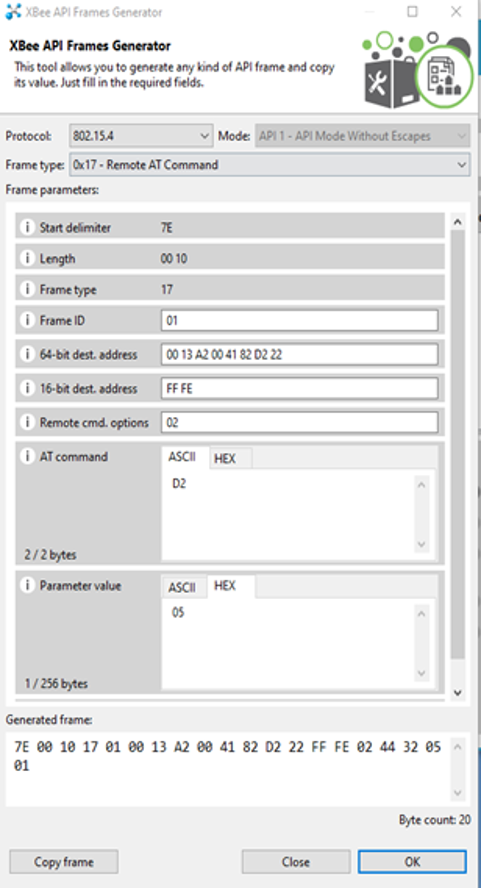
\includegraphics[width=\textwidth]{xctuFrames1.png}
			\caption{Turn On Pin 18}
		\end{subfigure}
		\begin{subfigure}[t]{0.22\textwidth}
			\centering
			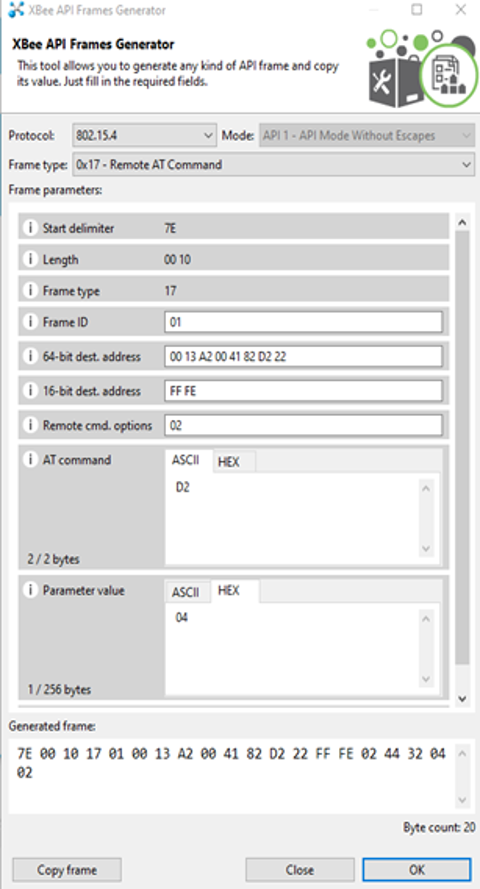
\includegraphics[width=\textwidth]{xctuFrames2.png}
			\caption{Turn Off Pin 18}
		\end{subfigure}
		\caption{API Frames created in XCTU}
	\end{figure} 
	\begin{lstlisting}
	#Configure AD2 and DIO2 to control pin-18
	
	import serial
	import binascii
	import time
	
	ser = serial.Serial(COM3)
	ser.baudrate = 9600
	
	#XCTU API Frame remote AT command used to control pin-18
	#Power ON
	turnOn = "7E 00 01 17 01 00 13 A2 00 41 82 D2 22 FF FE 02 44 32 05 01"
	#Power OFF
	turnOff = "7E 00 01 17 01 00 13 A2 00 41 82 D2 22 FF FE 02 44 32 04 02"
	
	#Use binascii to convert hex instruction to binary
	messageOn = "".join(turnOn.split()) 
	on = binascii.unhexlify(messageOn)
	
	messageOff = "".join(turnOff.split())
	off = binascii.unhexlify(messageOff)
	
	#Test write commands, flash led at 5 sec intervals
	count = 0
	while (count < 10)
		ser.write(on)
		time.sleep(5)
		ser.write(off)
		count = count + 1
	\end{lstlisting}